\section{连续性方程}
\label{sec:transp-continuity}

回到例~\ref{ex:transp-stretch}。三角形被$v=x$搬运到$t=\ln2$时，底变成了原来的两倍，高度不变，曲线下的面积从$1$变成了$2$。如果$u$表示粒子携带的标签，这没有问题；如果用它表示单位长度的墨水质量，总质量就凭空翻了一倍。质量不会凭空产生，所以墨水的浓度不满足输运方程，我们需要一个由质量平衡出发的新方程。

\paragraph{一维的质量平衡}
用$\rho(x,t)$表示单位长度的质量，取一段固定的区间$[a,b]$。流量$\rho v$是单位时间穿过某一点的质量，正号表示向右。如图~\ref{fig:transp-balance}(a)，区间内质量的变化等于从$a$流入的减去从$b$流出的，再加上区间内的源项$f$：
\[
  \frac{\mathrm{d}}{\mathrm{d}t}\int_a^{b}\rho\,\mathrm{d}x
  =\rho v\big|_{x=a}-\rho v\big|_{x=b}+\int_a^{b}f\,\mathrm{d}x.
\]

设$\rho$、$v$足够光滑，用微积分基本定理把两端的差写成积分：
\[
  \int_a^{b}\bigl(\partial_t\rho+\partial_x(\rho v)-f\bigr)\,\mathrm{d}x=0.
\]
区间是任取的，被积函数连续，所以它恒为零，这就是一维的连续性方程。

\begin{BookInlineFigure}
  \centering
  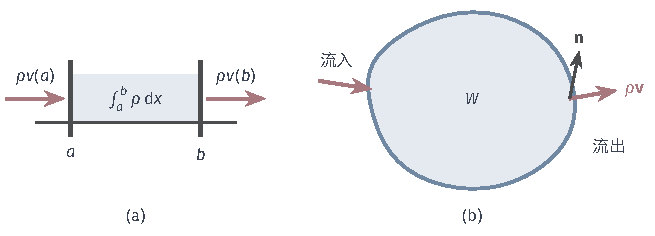
\includegraphics[width=111mm]{figures/06-differential-equations/02-partial-differential-equations/tikz/transp-balance/figure.pdf}
  \caption{控制区域的质量平衡。(a)区间$[a,b]$内的质量变化由两端的流量差决定。(b)平面区域$W$，红色箭头是质量流$\rho\bm{v}$，它在外法向$\bm{n}$上的投影为正时流出、为负时流入。}
  \label{fig:transp-balance}
\end{BookInlineFigure}

\paragraph{多维的质量平衡}
取固定的\term{控制区域}（control region）$W\subset\mathbb{R}^{d}$，如图~\ref{fig:transp-balance}(b)，边界光滑。穿过边界的质量流是$\rho\bm{v}\cdot\bm{n}$，于是
\begin{equation}
  \frac{\mathrm{d}}{\mathrm{d}t}\int_W\rho\,\mathrm{d}\bm{x}
  =-\int_{\partial W}\rho\bm{v}\cdot\bm{n}\,\mathrm{d}S+\int_Wf\,\mathrm{d}\bm{x}.
  \label{eq:transp-balance}
\end{equation}
由散度定理（见\BookChapterRef{chap:integral-theorems}{卷二第27章“积分定理”}），边界积分等于$\int_W\nabla\cdot(\rho\bm{v})\,\mathrm{d}\bm{x}$。由$W$的任意性，得到下面的方程。

\begin{definition}[连续性方程]
\label{def:transp-continuity}
给定速度场$\bm{v}$和源项$f$，未知密度$\rho(\bm{x},t)$满足的方程
\begin{equation}
  \partial_t\rho+\nabla\cdot(\rho\bm{v})=f
  \label{eq:transp-continuity}
\end{equation}
称为\term{连续性方程}（continuity equation）。
\end{definition}

把散度展开，可以看清它与输运方程的差别：
\begin{equation}
  \partial_t\rho+\bm{v}\cdot\nabla\rho=f-\rho\,\nabla\cdot\bm{v}.
  \label{eq:transp-divergence-correction}
\end{equation}
左端仍然是物质导数，右端多了一项$-\rho\nabla\cdot\bm{v}$，它就是散度修正。粒子携带的值不变，但$\rho$是“粒子周围的拥挤程度”，流动把周围的空间撑大或压小，这个量就要变。

当$\nabla\cdot\bm{v}=0$时修正项消失，两个方程完全一样，这样的速度场称为\term{无散度速度场}（divergence-free velocity field）。一般的速度场下两个方程不同，同一个初值走出的结果也不同。

\begin{example}[同一流动下的值与密度]
\label{ex:transp-rho-stretch}
仍取$v=x$，初值同式~\eqref{eq:transp-tent}。连续性方程是式~\eqref{eq:transp-reaction}的$c=\nabla\cdot v=1$情形，沿特征线的解是
\[
  \rho(x,t)=\mathrm{e}^{-t}\rho_0\bigl(x\mathrm{e}^{-t}\bigr).
\]

直接代入验证。对$t$求偏导，
\[
  \partial_t\rho=-\mathrm{e}^{-t}\rho_0-x\mathrm{e}^{-2t}\rho_0'.
\]
$\partial_x(x\rho)=\rho+x\partial_x\rho$，其中第一项是$\mathrm{e}^{-t}\rho_0$，第二项是$x\mathrm{e}^{-2t}\rho_0'$。两式相加为零。

点$(3,\ln2)$的出发位置是$1.5$。输运方程的解是$u(3,\ln2)=0.5$，连续性方程的解是
\[
  \rho(3,\ln2)=\tfrac12\cdot\rho_0(1.5)=0.25.
\]

积分验证总量。三角形的面积是$1$，时刻$t$时，对$\rho$换元$z=x\mathrm{e}^{-t}$，
\[
  \int_{\mathbb{R}}\rho(x,t)\,\mathrm{d}x=\int_{\mathbb{R}}\rho_0(z)\,\mathrm{d}z=1.
\]
同样的换元用在$u$上，多出的因子$\mathrm{e}^{t}$没有抵消，于是$\int u(x,t)\,\mathrm{d}x=\mathrm{e}^{t}$。
\end{example}

图~\ref{fig:transp-value-density}把这个例子放在一起比较。(a)和(b)的初值、流动完全相同，(a)中三角形的高度不变，面积翻倍；(b)中高度减半，面积不变。(c)是沿$x_0=1$这条特征线的三个量：$u$恒为$1$，体积倍率$J=\mathrm{e}^{t}$增长，密度$\rho=\mathrm{e}^{-t}$下降，乘积$\rho J$恒为$1$。

\begin{BookInlineFigure}
  \centering
  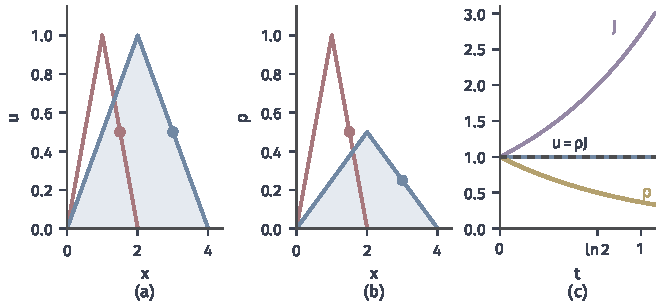
\includegraphics[width=112mm]{figures/06-differential-equations/02-partial-differential-equations/matplotlib/transp-value-density/figure.pdf}
  \caption{$v=x$，$t=\ln2$，初值同式~\eqref{eq:transp-tent}（红）。(a)场值$u$，浅蓝面积为$2$。(b)密度$\rho$，浅蓝面积为$1$，两图中的点都是$x_0=1.5$及其像。(c)沿$x_0=1$的特征线：$u$（蓝）、$\rho$（黄）、体积倍率$J$（紫）与乘积$\rho J$（虚线）。}
  \label{fig:transp-value-density}
\end{BookInlineFigure}

这里有两件容易混淆的事。沿轨迹密度不变，说的是物质导数为零，这只在$\nabla\cdot\bm{v}=0$时成立；总质量不变，说的是全空间的积分不随时间变化，它在$\bm{v}$不是无散度时同样成立，只要密度衰减足够快、没有质量从边界流失。例~\ref{ex:transp-rho-stretch}中总质量不变，沿轨迹的密度却在下降。

\subsection{体积变化}
\label{sec:transp-volume}

修正项$\rho\nabla\cdot\bm{v}$的来历，要从体积的变化说起。想象一维流动中相邻的两个粒子，相距$\Delta x$。前面的粒子比后面的多走了$\bigl(v(x+\Delta x)-v(x)\bigr)\,\mathrm{d}t$，所以它们的间距以$\partial_xv\,\Delta x$的速度增大，相对增长率就是$\partial_xv$。散度是这个现象在多维的写法。

\paragraph{Jacobian的演化}
记流映射的Jacobian行列式
\begin{equation}
  J_{s,t}(\bm{x})=\det\mathrm{D}\bm{\varphi}_{s,t}(\bm{x}).
  \label{eq:transp-jacobian}
\end{equation}

第~\ref{chap:ode-sensitivity}章证明了，Jacobian矩阵沿轨迹满足线性方程
\[
  \partial_t\mathrm{D}\bm{\varphi}_{s,t}=\nabla\bm{v}\bigl(\bm{\varphi}_{s,t},t\bigr)\,\mathrm{D}\bm{\varphi}_{s,t}.
\]
它的行列式满足Liouville公式，在这里的记号下，这个公式是
\begin{equation}
  \partial_tJ_{s,t}=\bigl(\nabla\cdot\bm{v}\bigr)\bigl(\bm{\varphi}_{s,t},t\bigr)\,J_{s,t},\qquad J_{s,s}=1,
  \label{eq:transp-liouville}
\end{equation}
解出来就是
\begin{equation}
  J_{s,t}(\bm{x})=\exp\int_s^{t}\bigl(\nabla\cdot\bm{v}\bigr)\bigl(\bm{\varphi}_{s,r}(\bm{x}),r\bigr)\,\mathrm{d}r>0.
  \label{eq:transp-liouville-solution}
\end{equation}

结合换元公式，可测集$\bm{W}$被搬运后的体积是$\int_{\bm{W}}J_{s,t}\,\mathrm{d}\bm{x}$。这说明$J_{s,t}$是局部的体积倍率，散度是体积倍率在瞬时的对数变化率。

\begin{example}[Logistic速度场的体积倍率]
\label{ex:transp-logistic-jacobian}
取$\Omega=(0,1)$，$v(x)=x(1-x)$，它正是第~\ref{chap:ode-sensitivity}章用过的Logistic方程的右端。流映射是
\[
  \varphi_{t}(x)=\frac{x\mathrm{e}^{t}}{1-x+x\mathrm{e}^{t}}.
\]
对$x$求导，
\[
  J_{0,t}(x)=\partial_x\varphi_{t}(x)=\frac{\mathrm{e}^{t}}{\bigl(1-x+x\mathrm{e}^{t}\bigr)^{2}}.
\]

$t=\ln2$时，$J_{0,\ln2}(x)=2/(1+x)^{2}$。取$x=1/3$，得到
\[
  J_{0,\ln2}(1/3)=\frac{2}{(4/3)^{2}}=\frac98.
\]

用式~\eqref{eq:transp-liouville-solution}核对。这条轨迹是$\varphi_s(1/3)=\mathrm{e}^{s}/(2+\mathrm{e}^{s})$，散度沿它取值$1-2\varphi_s$，积分得
\[
  \int_0^{\ln2}\Bigl(1-\frac{2\mathrm{e}^{s}}{2+\mathrm{e}^{s}}\Bigr)\mathrm{d}s
  =\ln2-2\ln\frac43=\ln\frac98.
\]
指数正好是$9/8$，与直接求导相同。
\end{example}

图~\ref{fig:transp-spreading}(a)从$[0,1]$上等间距的点出发画特征线。左半部分的线逐渐拉开，右半部分的线向$x=1$挤压，线的疏密直接反映出体积倍率。(b)是$t=\ln2$时的倍率$J_{0,\ln2}$：左边大于$1$，表示膨胀；右边小于$1$，表示压缩。绿点是用流映射的差分算出来的，与公式重合。

\begin{BookInlineFigure}
  \centering
  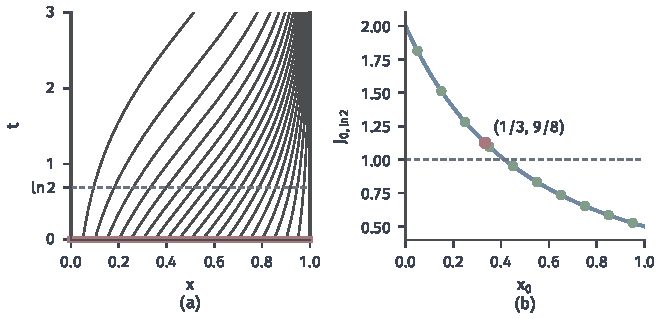
\includegraphics[width=112mm]{figures/06-differential-equations/02-partial-differential-equations/matplotlib/transp-spreading/figure.pdf}
  \caption{Logistic速度场$v=x(1-x)$。(a)从等间距的初始位置（红线）出发的特征线，两端的粗线是不动的边界。(b)$t=\ln2$的体积倍率（蓝），绿点是对流映射做中心差分的结果，红点是例~\ref{ex:transp-logistic-jacobian}的$(1/3,9/8)$，虚线是$J=1$。}
  \label{fig:transp-spreading}
\end{BookInlineFigure}

$\nabla\cdot\bm{v}\equiv0$时，由式~\eqref{eq:transp-liouville-solution}，$J_{s,t}\equiv1$，流映射保持体积。这是第~\ref{sec:transp-flow}节旋转场和鞍点场的共同之处。图~\ref{fig:transp-volume-flows}比较了三种平面流。

旋转场的散度是$\partial_1(-x_2)+\partial_2x_1=0$，鞍点场是$1-1=0$，面积都不变。放大场$\bm{v}=(x_1,x_2)^{\top}$的散度是$2$，$J=\mathrm{e}^{2t}$，$t=\ln2$时面积放大到$4$倍，$0.25$变成了$1$。一般的流要保留这个倍率，不能当作$1$。

\begin{BookInlineFigure}
  \centering
  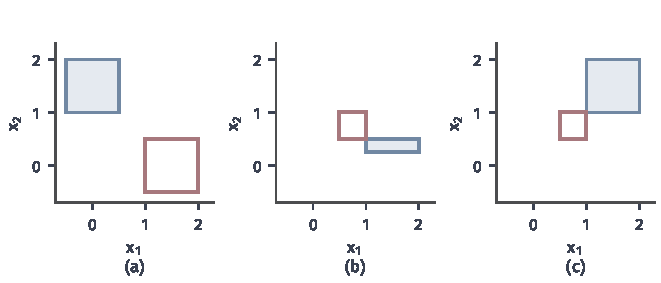
\includegraphics[width=112mm]{figures/06-differential-equations/02-partial-differential-equations/matplotlib/transp-volume-flows/figure.pdf}
  \caption{正方形（红框）被流映射搬运后的像（浅蓝）。(a)旋转场，$t=\pi/2$，面积$1$不变。(b)鞍点场，$t=\ln2$，正方形变成长方形，面积仍为$0.25$。(c)放大场，$t=\ln2$，面积由$0.25$变为$1$。}
  \label{fig:transp-volume-flows}
\end{BookInlineFigure}

\subsection{密度搬运}
\label{sec:transp-density}

有了体积倍率，可以直接算出密度。如图~\ref{fig:transp-pushforward}，一小块区域$\bm{W}$里的质量是$m\approx\rho_0(\bm{x})\lvert\bm{W}\rvert$。流动把它带到$\bm{\varphi}_{0,t}(\bm{W})$，质量不变，体积乘上了$J_{0,t}(\bm{x})$，所以新的密度应当是$\rho_0(\bm{x})/J_{0,t}(\bm{x})$。

\begin{BookInlineFigure}
  \centering
  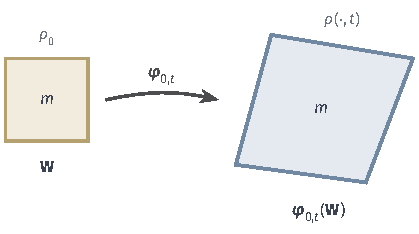
\includegraphics[width=70.9mm]{figures/06-differential-equations/02-partial-differential-equations/tikz/transp-pushforward/figure.pdf}
  \caption{一小块质量被流映射搬运。质量$m$不变，体积变为$J_{0,t}$倍，所以密度除以$J_{0,t}$。}
  \label{fig:transp-pushforward}
\end{BookInlineFigure}

\paragraph{推前测度}
这个想法用测度来说最干净。记初始质量分布为$\mu_0$，$\mathrm{d}\mu_0=\rho_0\,\mathrm{d}\bm{x}$。时刻$t$落在集合$B$中的质量，正好是初始时刻位于$\bm{\varphi}_{t,0}(B)$中的质量，于是
\begin{equation}
  \mu_t(B)=\mu_0\bigl(\bm{\varphi}_{t,0}(B)\bigr),\qquad
  \mu_t=(\bm{\varphi}_{0,t})_{\#}\mu_0.
  \label{eq:transp-pushforward-measure}
\end{equation}
也就是说，$\mu_t$是$\mu_0$在流映射下的推前测度，定义和基本性质见\BookChapterRef{chap:pushforward-measures}{卷四第9章“推前测度”}。

\begin{theorem}[密度搬运公式]
\label{thm:transp-density}
设$\bm{v}$满足条件（V），$\nabla\cdot\bm{v}$关于$\bm{x}$连续可微且偏导数连续，$\rho_0\in C^{1}(\mathbb{R}^{d})$。则方程~\eqref{eq:transp-continuity}（$f=0$）有唯一满足$\rho(\cdot,0)=\rho_0$的$C^{1}$解，它由下式确定：
\begin{equation}
  \rho\bigl(\bm{\varphi}_{0,t}(\bm{x}),t\bigr)\,J_{0,t}(\bm{x})=\rho_0(\bm{x}).
  \label{eq:transp-density}
\end{equation}
进而对任意非负可测函数$h$，有
\begin{equation}
  \int_{\mathbb{R}^{d}}\rho(\bm{y},t)\,h(\bm{y})\,\mathrm{d}\bm{y}
  =\int_{\mathbb{R}^{d}}\rho_0(\bm{x})\,h\bigl(\bm{\varphi}_{0,t}(\bm{x})\bigr)\,\mathrm{d}\bm{x}.
  \label{eq:transp-pushforward}
\end{equation}
若$\rho_0\geq0$，则$\rho\geq0$；取$h=1$，总质量不随时间变化。
\end{theorem}

\begin{proof}
设$\rho$是$C^{1}$解。沿轨迹，由式~\eqref{eq:transp-along}和式~\eqref{eq:transp-liouville}，
\[
  \frac{\mathrm{d}}{\mathrm{d}t}\Bigl[\rho\bigl(\bm{\varphi}_{0,t}(\bm{x}),t\bigr)J_{0,t}(\bm{x})\Bigr]
  =\bigl(\partial_t\rho+\bm{v}\cdot\nabla\rho+\rho\nabla\cdot\bm{v}\bigr)\bigl(\bm{\varphi}_{0,t}(\bm{x}),t\bigr)\,J_{0,t}(\bm{x}).
\]
括号里正是$\partial_t\rho+\nabla\cdot(\rho\bm{v})=0$，所以$\rho J$沿轨迹不变，取$t=0$的值即得式~\eqref{eq:transp-density}，唯一性得证。

反过来，令$R(\bm{x},t)=\rho_0(\bm{x})/J_{0,t}(\bm{x})$。$\nabla\cdot\bm{v}$关于$\bm{x}$是$C^{1}$的，由式~\eqref{eq:transp-liouville-solution}，$J_{0,t}$关于$(\bm{x},t)$是$C^{1}$的且恒正，$R$也是。沿定理~\ref{thm:transp-classical}证明中的映射$\bm{\Psi}$，定义$\rho=R\circ\bm{\Psi}^{-1}$，它是$C^{1}$的，并满足式~\eqref{eq:transp-density}。再用上面的等式把导数读出来，由$J_{0,t}>0$和$\bm{\Psi}$是满射，方程在每一点成立。

式~\eqref{eq:transp-pushforward}由换元$\bm{y}=\bm{\varphi}_{0,t}(\bm{x})$得到。换元产生因子$J_{0,t}$，由式~\eqref{eq:transp-density}，被积函数中$\rho J$恰好等于$\rho_0$：
\[
  \begin{aligned}
  \int\rho(\bm{y},t)h(\bm{y})\,\mathrm{d}\bm{y}
  &=\int\rho\bigl(\bm{\varphi}_{0,t}(\bm{x}),t\bigr)h\bigl(\bm{\varphi}_{0,t}(\bm{x})\bigr)J_{0,t}(\bm{x})\,\mathrm{d}\bm{x}\\
  &=\int\rho_0(\bm{x})h\bigl(\bm{\varphi}_{0,t}(\bm{x})\bigr)\,\mathrm{d}\bm{x}.
  \end{aligned}
\]
非负性由式~\eqref{eq:transp-density}和$J_{0,t}>0$得到。
\end{proof}

式~\eqref{eq:transp-density}是本章的核心：密度倍率$1/J$与体积倍率$J$逐点抵消，乘积沿轨迹不变。取$h$为集合$B$的指示函数，式~\eqref{eq:transp-pushforward}就是式~\eqref{eq:transp-pushforward-measure}。定理还要求$\nabla\cdot\bm{v}$对$\bm{x}$可微，这是为了得到$C^{1}$解；只求弱解时可以去掉，见第~\ref{sec:transp-weak}节。

有源项时，同样的计算给出$\frac{\mathrm{d}}{\mathrm{d}t}[\rho J]=fJ$，沿轨迹积分得到
\begin{equation}
  \rho\bigl(\bm{\varphi}_{0,t}(\bm{x}),t\bigr)\,J_{0,t}(\bm{x})
  =\rho_0(\bm{x})+\int_0^{t}f\bigl(\bm{\varphi}_{0,s}(\bm{x}),s\bigr)\,J_{0,s}(\bm{x})\,\mathrm{d}s.
  \label{eq:transp-density-source}
\end{equation}

\begin{example}[区间上的密度搬运]
\label{ex:transp-logistic-density}
在$(0,1)$上取$v=x(1-x)$，初始密度$\rho_0=1$。由例~\ref{ex:transp-logistic-jacobian}的结果，逆流映射是
\[
  \varphi_{t,0}(y)=\frac{y\mathrm{e}^{-t}}{1-y+y\mathrm{e}^{-t}}.
\]

把$J_{0,t}$用当前位置$y$表示。令$D=1-y+y\mathrm{e}^{-t}$，代入得$1-x+x\mathrm{e}^{t}=1/D$，于是$J_{0,t}=\mathrm{e}^{t}D^{2}$。由式~\eqref{eq:transp-density}，
\[
  \rho(y,t)=\frac{\mathrm{e}^{-t}}{\bigl(1-y+y\mathrm{e}^{-t}\bigr)^{2}}.
\]

取$t=\ln2$，$y=1/2$。出发位置是$x=\varphi_{\ln2,0}(1/2)=1/3$，倍率是$9/8$，所以
\[
  \rho(1/2,\ln2)=\frac{8}{9}.
\]
代入上面的公式核对：$D=3/4$，$\rho=\tfrac12\cdot\tfrac{16}{9}=\tfrac89$。

再验证总质量。$t=\ln2$时$\rho(y,\ln 2)=\tfrac12(1-y/2)^{-2}$，
\[
  \int_0^{1}\frac12\Bigl(1-\frac{y}{2}\Bigr)^{-2}\mathrm{d}y=\Bigl[\frac{1}{1-y/2}\Bigr]_0^{1}=2-1=1.
\]
\end{example}

图~\ref{fig:transp-logistic-density}(a)是这个密度在不同时刻的形状。均匀的初始分布逐渐向右端集中，绿色直方图是$40000$个按初始分布抽取的粒子在$t=\ln4$的位置，与公式吻合。

(b)从另一个角度看。质量$\int_0^{y}\rho\,\mathrm{d}x$等于初始时位于$(0,\varphi_{t,0}(y))$中的质量，而$\rho_0=1$，所以累积质量恰好是逆流映射本身。$t=\ln2$时，左半区间的质量是$\varphi_{\ln2,0}(1/2)=1/3$。

\begin{BookInlineFigure}
  \centering
  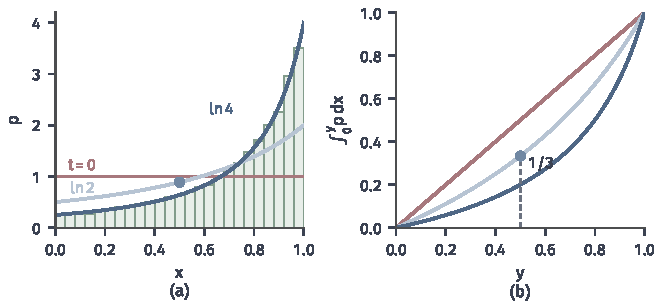
\includegraphics[width=112mm]{figures/06-differential-equations/02-partial-differential-equations/matplotlib/transp-logistic-density/figure.pdf}
  \caption{$(0,1)$上$v=x(1-x)$对均匀密度的搬运。(a)密度$\rho$：$t=0$（红）、$t=\ln2$与$t=\ln4$（蓝色由浅到深），绿色直方图是$40000$个粒子（固定种子）在$t=\ln4$的分布，蓝点是$(1/2,8/9)$。(b)累积质量，蓝点表示$t=\ln2$时左半区间的质量为$1/3$。}
  \label{fig:transp-logistic-density}
\end{BookInlineFigure}

平面上的情形相同。图~\ref{fig:transp-density-2d}把一个Gaussian形的密度分别交给三种流，运行时间都是$t=1$，初始峰值是$1$。放大场$\bm{v}=\bm{x}/2$的散度是$1$，峰值降到$\mathrm{e}^{-1}\approx0.37$；鞍点场$\bm{v}=(x_1/2,-x_2/2)^{\top}$的散度是$0$，形状变了，峰值不变；收缩场$\bm{v}=-\bm{x}/2$的散度是$-1$，峰值升到$\mathrm{e}\approx2.72$。

\begin{BookInlineFigure}
  \centering
  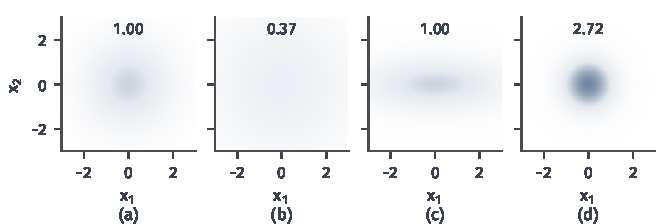
\includegraphics[width=112mm]{figures/06-differential-equations/02-partial-differential-equations/matplotlib/transp-density-2d/figure.pdf}
  \caption{同一Gaussian形密度的搬运，蓝色越深密度越大，图中数字是峰值。(a)初值。(b)放大场，$t=1$。(c)无散度的鞍点场，$t=1$。(d)收缩场，$t=1$。四幅图共用一个色阶。}
  \label{fig:transp-density-2d}
\end{BookInlineFigure}

概率密度是这里的特例：$\rho_0\geq0$且总质量为$1$。定理~\ref{thm:transp-density}说明这两条性质都被流保持，所以时刻$t$的$\rho$仍是概率密度，$\bm{\varphi}_{0,t}$就是随机变量的变换。除此之外，归一化没有增加任何东西，这里讨论的是一般的守恒密度。

表~\ref{tab:transp-value-density}把两种量并排列出。

\begin{BookInlineTable}
  \centering
  \caption{沿轨迹的场值与密度的比较。设$\bm{v}$满足条件（V），无源项。}
  \label{tab:transp-value-density}
  \begin{tabular}{p{16mm}p{42mm}p{42mm}}
    \toprule
    & 场值$u$ & 密度$\rho$ \\
    \midrule
    方程 & $\partial_tu+\bm{v}\cdot\nabla u=0$ & $\partial_t\rho+\nabla\cdot(\rho\bm{v})=0$ \\
    沿轨迹 & $u$不变 & $\rho J$不变 \\
    解 & $u_0\circ\bm{\varphi}_{t,0}$ & $(\rho_0/J_{0,t})\circ\bm{\varphi}_{t,0}$ \\
    不变量 & 最大值、最小值 & 总质量 \\
    例$v=x$，$t=\ln2$ & 高度不变，面积翻倍 & 高度减半，面积不变 \\
    \bottomrule
  \end{tabular}
\end{BookInlineTable}

\subsection{边界通量}
\label{sec:transp-boundary-flux}

全空间上质量不变，是因为没有地方可去。在有界区域里，粒子可能离开，也可能有新的粒子进入，总质量的变化完全由边界决定。

\paragraph{流入、流出与无通量}
在式~\eqref{eq:transp-balance}中取$W=\Omega$，把边界分成三部分：
\begin{equation}
  \Gamma_{-}=\{\bm{v}\cdot\bm{n}<0\},\qquad
  \Gamma_{+}=\{\bm{v}\cdot\bm{n}>0\},\qquad
  \Gamma_{0}=\{\bm{v}\cdot\bm{n}=0\}.
  \label{eq:transp-boundary-parts}
\end{equation}
图~\ref{fig:transp-boundary-parts}是匀速水平流过圆盘时的三部分。$\Gamma_{-}$上给定密度$\rho=g$（质量随粒子进入），$\Gamma_{+}$上的值由内部决定，$\Gamma_{0}$上没有流量。

总质量$M(t)=\int_\Omega\rho\,\mathrm{d}\bm{x}$的变化率是
\begin{equation}
  M'(t)=\int_{\Gamma_{-}}g\,\lvert\bm{v}\cdot\bm{n}\rvert\,\mathrm{d}S
  -\int_{\Gamma_{+}}\rho\,\bm{v}\cdot\bm{n}\,\mathrm{d}S
  +\int_\Omega f\,\mathrm{d}\bm{x}.
  \label{eq:transp-mass-rate}
\end{equation}

\begin{BookInlineFigure}
  \centering
  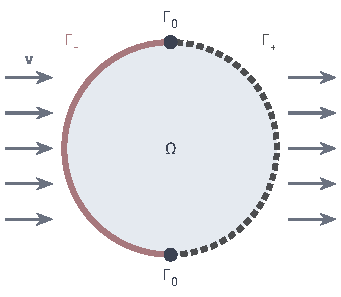
\includegraphics[width=57.8mm]{figures/06-differential-equations/02-partial-differential-equations/tikz/transp-boundary-parts/figure.pdf}
  \caption{速度场$\bm{v}=(1,0)^{\top}$（灰色箭头）下，圆盘的边界分成三部分：红色实线是入流边界$\Gamma_{-}$，深灰虚线是出流边界$\Gamma_{+}$，上下两点是$\bm{v}\cdot\bm{n}=0$的$\Gamma_{0}$。}
  \label{fig:transp-boundary-parts}
\end{BookInlineFigure}

下面在$(0,1)$上取$\rho_0=1$，看三个例子，$M(0)=1$。

第一，$v=1$，$g=0$。这时$\rho(x,t)=1$（$x>t$）、$\rho=0$（$x<t$）。质量以单位速率从右端流出，所以
\[
  M(t)=\max\{1-t,\ 0\}.
\]
式~\eqref{eq:transp-mass-rate}的流出项在$t<1$时等于$\rho(1,t)\cdot1=1$，符合$M'=-1$。

第二，$v=x-1/2$，两端都是出流。解是$\rho=\mathrm{e}^{-t}$，代入验证：
\[
  \partial_t\rho=-\mathrm{e}^{-t},\qquad \partial_x\bigl(\rho\,(x-\tfrac12)\bigr)=\mathrm{e}^{-t}.
\]
两端的流出量都是$\tfrac12\mathrm{e}^{-t}$，合起来恰好是$M'=-\mathrm{e}^{-t}$，因此
\[
  M(t)=\mathrm{e}^{-t}.
\]

第三，$v=x(1-x)$，两端$v=0$，边界是无通量的。例~\ref{ex:transp-logistic-density}中质量向右端堆积，但始终没有离开区间，
\[
  M(t)=1.
\]

这三种情形对应图~\ref{fig:transp-mass-balance}。把第一例换成$g=2$，则$t<1$时左端流入$2$、右端流出$1$，$M=1+t$；$t\geq1$时整个区间密度为$2$，进出相等，$M=2$。

\begin{BookInlineFigure}
  \centering
  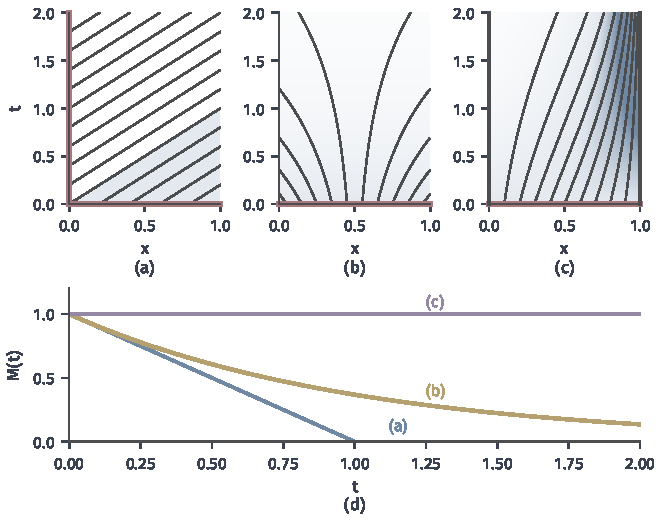
\includegraphics[width=112mm]{figures/06-differential-equations/02-partial-differential-equations/matplotlib/transp-mass-balance/figure.pdf}
  \caption{$(0,1)$上的质量平衡，$\rho_0=1$。上排是特征线（深灰）和密度（蓝色越深越大）：(a)$v=1$，入流数据为$0$；(b)$v=x-1/2$，两端出流；(c)$v=x(1-x)$，两端无通量（粗线）。红线是给数据的边界。(d)三种情形的总质量$M(t)$。}
  \label{fig:transp-mass-balance}
\end{BookInlineFigure}

质量守恒是一个有条件的结论。只有当右端全部为零时，$M$才不变，典型条件是$\Omega$封闭，即$\partial\Omega$上$\bm{v}\cdot\bm{n}=0$，并且没有源项。此时轨迹不会穿过边界，流映射把$\Omega$映到自身，定理~\ref{thm:transp-density}的论证可以在$\Omega$上进行，例~\ref{ex:transp-logistic-density}就是这样。否则，全空间上的守恒结论不能照搬到有界区域。
